% Copyright 2004 by Till Tantau <tantau@users.sourceforge.net>.

\title{Negative Selection Algorithm}

\author{Li Meizhen}

\institute[College of Argriculture and Biotechnology] % (optional, but mostly needed)
{
  College of Argriculture and Biotechnology\\
  Zhejiang University
}

\date{March 29th, 2018}

% Delete this, if you do not want the table of contents to pop up at
% the beginning of each subsection:
\AtBeginSubsection[]
{
  \begin{frame}<beamer>{Outline of NSA}
    \tableofcontents[currentsection,currentsubsection]
  \end{frame}
}

% Let's get started
%\begin{document}

\begin{frame}
  \titlepage
  \end{frame}


\begin{frame}{Outline of Negative Selection Algorithm}
  \tableofcontents
  % You might wish to add the option [pausesections]
\end{frame}

% Section and subsections will appear in the presentation overview
% and table of contents.
\section{Introduction of NSA}

\subsection{Inspiration}

\begin{frame}{Biological immune system}
  \begin{itemize}
  \item {
    The antigen-antibody reaction is an exclusive process.
  }
  \item {
    The primary role of immune system is to distinguish self from non-self.
  }
  \item {
    Immune cells are tolerant to self antigens but activate defense mechanisms when recognize non-self antigens.   
  }
  \item {
    The negative selection of T cells happened in the thymus during maturation.
  }
  \end{itemize}
\end{frame}

\begin{frame}{Biological immune system}
  \begin{figure}[hb]
  \centering
  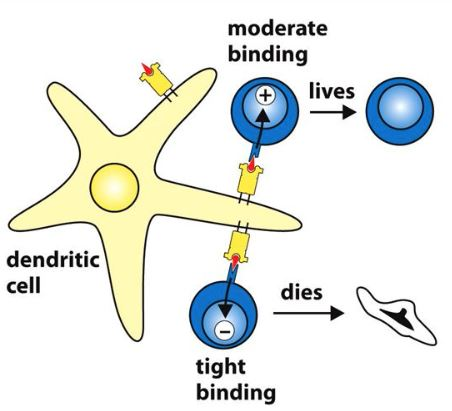
\includegraphics[width=0.6\textwidth]{NSA/figures/NST.JPG}
  \caption{Negative selection of T cells}
  \end{figure}
\end{frame}

\begin{frame}{Biological immune system}
  \begin{figure}[hb]
  \centering
  \includegraphics[width=0.6\textwidth]{NSA/figures/is.jpg}
  \caption{Antigen-antibody interaction}
  \end{figure}
\end{frame}


\subsection{Definition}

% You can reveal the parts of a slide one at a time
% with the \pause command:
\begin{frame}{Defining the NSA}
  \begin{itemize}
  \item<1->{
    Define Self as a normal pattern of activity or stable behavior of a system/process.\\
    -Represent the collection as multiset of S of strings of length \emph{l} over a finite alphabet.
  }
  \item<2-> {   
    Generate a set R of detectors,each of which fails to match any string in S.
  }
  % You can also specify when the content should appear
  % by using <n->:
  
  \end{itemize}
\end{frame}
 
\begin{frame}{Flowchart}
  \begin{figure}[hb]
  \centering
  \includegraphics[width=0.8\textwidth]{NSA/figures/flowchart1.jpg}
  \caption{Generation of effective detector}
  \end{figure}
\end{frame}

\begin{frame}{Defining the NSA}
  \begin{itemize}
  \item {
    Monitor new observations for changes by continually testing the detectors matching against representatives of S.  If any detector ever matches, a change must have occurred in system behavior.
  }
  \end{itemize}
\end{frame}

\begin{frame}{Flowchart}
  \begin{figure}[hb]
  \centering
  \includegraphics[width=0.8\textwidth]{NSA/figures/flowchart2.jpg}
  \caption{Self-monitoring}
  \end{figure}
\end{frame}

\section{Second Main Section}

\subsection{Another Subsection}

\begin{frame}{Blocks}
\begin{block}{Block Title}
You can also highlight sections of your presentation in a block, with it's own title
\end{block}
\begin{theorem}
There are separate environments for theorems, examples, definitions and proofs.
\end{theorem}
\begin{example}
Here is an example of an example block.
\end{example}
\end{frame}

% Placing a * after \section means it will not show in the
% outline or table of contents.
\section*{Summary}

\begin{frame}{Summary}
  \begin{itemize}
  \item
    The \alert{first main message} of your talk in one or two lines.
  \item
    The \alert{second main message} of your talk in one or two lines.
  \item
    Perhaps a \alert{third message}, but not more than that.
  \end{itemize}
  
  \begin{itemize}
  \item
    Outlook
    \begin{itemize}
    \item
      Something you haven't solved.
    \item
      Something else you haven't solved.
    \end{itemize}
  \end{itemize}
\end{frame}



% All of the following is optional and typically not needed. 
\appendix
\section<presentation>*{\appendixname}
\subsection<presentation>*{For Further Reading}

\begin{frame}[allowframebreaks]
  \frametitle<presentation>{For Further Reading}
    
  \begin{thebibliography}{10}
    
  \beamertemplatebookbibitems
  % Start with overview books.

  \bibitem{Author1990}
    A.~Author.
    \newblock {\em Handbook of Everything}.
    \newblock Some Press, 1990.
 
    
  \beamertemplatearticlebibitems
  % Followed by interesting articles. Keep the list short. 

  \bibitem{Someone2000}
    S.~Someone.
    \newblock On this and that.
    \newblock {\em Journal of This and That}, 2(1):50--100,
    2000.
  \end{thebibliography}
\end{frame}

\end{document}


